%%%%%%%%%%%%%%%%%%%%%%%%%%%%%%%%%%%%%%%%%
% Journal Article
% LaTeX Template
% Version 1.3 (9/9/13)
%
% This template has been downloaded from:
% http://www.LaTeXTemplates.com
%
% Original author:
% Frits Wenneker (http://www.howtotex.com)
%
% License:
% CC BY-NC-SA 3.0 (http://creativecommons.org/licenses/by-nc-sa/3.0/)
%
%%%%%%%%%%%%%%%%%%%%%%%%%%%%%%%%%%%%%%%%%

%----------------------------------------------------------------------------------------
%	PACKAGES AND OTHER DOCUMENT CONFIGURATIONS
%----------------------------------------------------------------------------------------

\documentclass[twoside]{article}

\usepackage{lipsum} % Package to generate dummy text throughout this template
\usepackage{graphicx}

\usepackage[sc]{mathpazo} % Use the Palatino font
\usepackage[T1]{fontenc} % Use 8-bit encoding that has 256 glyphs
\linespread{1.05} % Line spacing - Palatino needs more space between lines
\usepackage{microtype} % Slightly tweak font spacing for aesthetics

\usepackage[hmarginratio=1:1,top=32mm,columnsep=20pt]{geometry} % Document margins
\usepackage{multicol} % Used for the two-column layout of the document
\usepackage[hang, small,labelfont=bf,up,textfont=it,up]{caption} % Custom captions under/above floats in tables or figures
\usepackage{booktabs} % Horizontal rules in tables
\usepackage{float} % Required for tables and figures in the multi-column environment - they need to be placed in specific locations with the [H] (e.g. \begin{table}[H])
\usepackage{hyperref} % For hyperlinks in the PDF

\usepackage{lettrine} % The lettrine is the first enlarged letter at the beginning of the text
\usepackage{paralist} % Used for the compactitem environment which makes bullet points with less space between them

\usepackage{abstract} % Allows abstract customization
\renewcommand{\abstractnamefont}{\normalfont\bfseries} % Set the "Abstract" text to bold
\renewcommand{\abstracttextfont}{\normalfont\small\itshape} % Set the abstract itself to small italic text

\usepackage{titlesec} % Allows customization of titles
\renewcommand\thesection{\Roman{section}} % Roman numerals for the sections
\renewcommand\thesubsection{\Roman{subsection}} % Roman numerals for subsections
\titleformat{\section}[block]{\large\scshape\centering}{\thesection.}{1em}{} % Change the look of the section titles
\titleformat{\subsection}[block]{\large}{\thesubsection.}{1em}{} % Change the look of the section titles

\usepackage{fancyhdr} % Headers and footers
\pagestyle{fancy} % All pages have headers and footers
\fancyhead{} % Blank out the default header
\fancyfoot{} % Blank out the default footer
%\fancyhead[C]{Running title $\bullet$ November 2012 $\bullet$ Vol. XXI, No. 1} % Custom header text
\fancyfoot[RO,LE]{\thepage} % Custom footer text

\usepackage{amsmath}

%----------------------------------------------------------------------------------------
%	TITLE SECTION
%----------------------------------------------------------------------------------------

\title{\vspace{-15mm}\fontsize{24pt}{10pt}\selectfont\textbf{Article Title}} % Article title

\author{
\large
\textsc{John Smith}\thanks{A thank you or further information}\\[2mm] % Your name
\normalsize University of California \\ % Your institution
\normalsize \href{mailto:john@smith.com}{john@smith.com} % Your email address
\vspace{-5mm}
}
\date{}

%----------------------------------------------------------------------------------------

\begin{document}

\maketitle % Insert title

\thispagestyle{fancy} % All pages have headers and footers

%----------------------------------------------------------------------------------------
%	ABSTRACT
%----------------------------------------------------------------------------------------

\begin{abstract}

\noindent \lipsum[1] % Dummy abstract text

\end{abstract}

%----------------------------------------------------------------------------------------
%	ARTICLE CONTENTS
%----------------------------------------------------------------------------------------

\begin{multicols}{2} % Two-column layout throughout the main article text

\chapter{Introduction}
Goal

\section{Reading guide}
The report should be seen as four sections, introduction, methods, results and conclusion.\\
The introduction covers the specification of the project by project formulation, system description, requirement specification and project scope.\\
Methods explains the approach to the project and solutions, planning and scheduling, work distribution and project structure.\\
The results covers the result of the project namely what have been made and what have been learned. Most subjects here will be described briefly but further information can be found in the more detailed descriptions in the documentation found on the CD.\\
The conclusion rounds up the project and weighs of expectations and goals.

\section{Glossary and abbreviations}
This section contains all the abbreviations and terms used in this project. The full name will often be written the first time an abbreviation is encountered.\\
The abbreviations and terms are general for the entire project and might not be used in this documents.
\begin{table}[H]
\centering
\begin{tabular}{|p{4cm}|p{7cm}|}
\hline
Term/abbreviation & Definition\\ \hline
PC / computer & General term for a computer / Personal Computer.\\ \hline
\end{tabular}
\end{table}
\section{Data Gathering}
The data used in this project was gathered by recording three different persons reading the same article from the website "www.tv2.dk". The voices was recorded using the software Audacity\footnote{http://sourceforge.net/projects/audacity/} and the Lame mp3 codex\footnote{http://lame.sourceforge.net/}. The data is then imported into matlab using the function \texttt{[data, Fs] = audioread(pathToFile)}. The data is then normalised by removing the mean of the data, and whitening the data. The files are in stereo and both channels are used by appending one channel to the other so to have one long array of data.

\section{Feature Extraction}
The Mel Frequency Cepstral Coefficient method is commonly used to extract features in speech and speaker recognition. The methods provides features that are useful for classifying linguistic content. The basis is that the speech from humans is uniquely filtered by the shape of the vocal tract, tongue, teeth etc\footnote{http://practicalcryptography.com/miscellaneous/machine-learning/guide-mel-frequency-cepstral-coefficients-mfccs/ - retrieved 4 june 2015}. 

MFCCs are found using a series of steps as can be seen in figure \ref{fig:MFCCsteps}.
\begin{figure}[H]
\centering
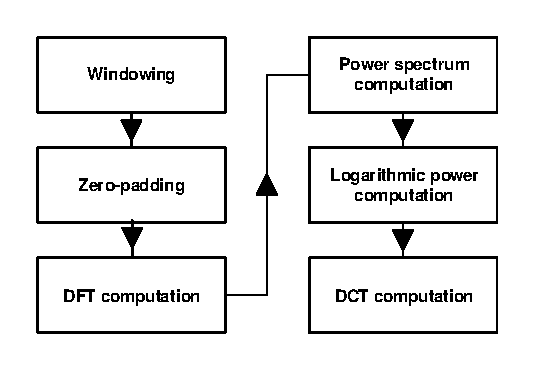
\includegraphics[scale=1]{billeder/MFCCsteps}
\caption{MFCC steps}
\label{fig:MFCCsteps}
\end{figure}
The figure has been derived from the article \cite{Sahidullah2012}. The steps can be described as follows:
\begin{enumerate}
\item Windowing: The speech signal is windows with either a Hamming or Hanning window.
\item Zero-padding: A number of zeros are padded to he windowed speech signal in order to enable fast Fourier transform (FFT).
\item DFT: The windowed speech signal is discrete fourier transformed using a FFT algorithm.
\item Power spectrum: The resulting spectrum is mapped onto the mel scale but utilising a triangular filter bank.
\item Logarithmic power: The power spectrum is converted to logarithmic scale with respect to the mel frequencies.
\item DCT: The logarithmic mel powers are discrete cosine transformed. The MFCCs is the amplitudes of the output spectrum.
\end{enumerate}

In MATLAB this is done using the toolbox, voicebox\footnote{http://www.ee.ic.ac.uk/hp/staff/dmb/voicebox/voicebox.html - retrieved 6 june 2015}. The function for getting the MFCCs is called \texttt{melcepst} and a thorough explaination can be found on the voicebox website\footnote{http://www.ee.ic.ac.uk/hp/staff/dmb/voicebox/doc/voicebox/melcepst.html}. 

In short the function is invoked like this:
\begin{verbatim}
mel = melcepst(data(:,i), Fs(i), 'M0d', nc, p, n, inc);
\end{verbatim}
With \textbf{data} being the signal we want to extract the MFCCs from. 
\textbf{Fs} is the sampling frequency of the signal. 
\textbf{'M0d'} is the mode string and the three characters correspond to Hamming window, include 0'th order cepstral coefficient and include delta coefficients.
\textbf{nc} is the number of cepstral coefficients excluding 0'th coefficient.
\textbf{p} is the number of filters in the filterbank.
\textbf{n} is the length of the frame in the samples.
and lastly \textbf{inc} is the frame increment value.
\fxnote{Possible formatting of this block of text}

In this project the window size is chosen to be 200 milliseconds. The default value for speaker recognition is 150 milliseconds while speech recognition is typically lower than that. The number of cepstral coefficients was chosen to be 30.

The mel output from the function is used for features. The resulting matrix is $M \times N$ with M being number of samples of each MFCC and N being number of MFCCs. For the data used in this project his corresponds to a $2175 \times 62$.


%------------------------------------------------
%!TEX root = ..\Master.tex

\section{Dimensionality Reduction}

e.g. finding projection vectors, choosing number of components, applications.\\

motivation:
data compression
speed up learning algorithm


\subsection{PCA}

Principal component analysis is used for reducing the number of dimensions of a feature space.
It works by projecting the data in the feature space, down to a fewer dimensional feature space by minimizing the squared projection error.
The reduced feature space does not nessecarily share the same features, but new features are found which best retains the variance in the data.

PCA should mainly be used for compressing the data to save memory or reducing running time of learning algorithm.
By reducing the amount of features most machine learning algorithms runs faster.
PCA can also be used to prevent overfitting, but its usually better to use regularization. \\

Figure \ref{fig:pca} shows a 3 dimensional feature space where all the data, within a small margin, lies in a 2 dimensional plane.
PCA is used to find two vectors $u^{(1)}$ and $u^{(2)}$ which spans this 2D plane.

\begin{figure}[H]
\centering
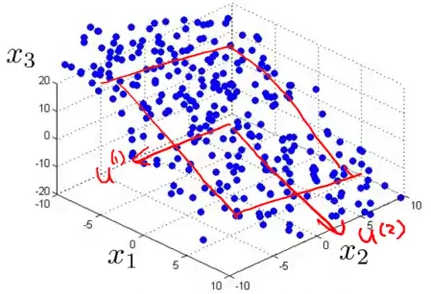
\includegraphics{billeder/pca}
\caption{3D to 2D pca illustration}
\label{fig:pca}
\end{figure}


Preprocessing of the data should be done before doing PCA. \\
Given the training set:
\begin{equation}
x = 
\begin{bmatrix}
x_1 & x_2 & \dots & x_m
\end{bmatrix}
\end{equation}

Ensure that every feature has zero mean by doing mean normalization:
\begin{equation}
\mu_j = \frac{1}{m} \sum^m_{i=1} x_j^{(i)}
\end{equation}
\begin{equation}
x_j = x_j - \mu_j
\end{equation}

Feature scaling can also be done if the features have very different value ranges. TODO \\

After preprocessing the data, we can do PCA on it.\\
We start by computing the covariance matrix $\Sigma$:
\begin{equation}
\Sigma = \frac{1}{m} \sum^n_{i=1} x^{(i)} {x^{(i)}}^T
\end{equation}

The covariance matrix descripes how the different features relates.
When doing feature reduction we want to remove features which has high correlation with other features.
An example could be a feature which descripes a length in cm and another feature descriping the same length in inches.
These features will have very high correlation and one of them can be removed from the feature space without loosing much information. \\

Then we compute the eigenvectors of covariance matrix:
\begin{equation}
U = \begin{bmatrix}
   u^{(1)} & u^{(2)} & \dots & u^{(n)}
 \end{bmatrix}
\in \mathbb{R}^{n \times n}
\end{equation}

The eigenvectors will lay in the directions of most variance in the data.
This is what is shown on Figure \ref{fig:pca}.
The longer the eigenvector, the more variance it descripes.
Therefore we want to keep the longest eigenvectors and remove the shortest eigenvectors.

The eigenvectors are ordered by length in the matrix $U$.
The longest is the first. \\

We select the first $k$ eigenvectors to get the reduced set of eigenvectors:
\begin{equation}
U_{reduce} = \begin{bmatrix}
   u^{(1)} & u^{(2)} & \dots & u^{(k)}
 \end{bmatrix}
\end{equation}

We can now calculate the new feature vectors:
\begin{equation}
z = U_{reduce}^Tx
\end{equation}

We have now reduced the feature space to a $k$ dimensional feature space.
Say we want to retain at least $95\%$ of the variance in the data.
We do this by picking the smallest value of $k$ so that:
\begin{equation}
\frac{\displaystyle\sum^{k}_{i=1} S_{ii}}{\displaystyle\sum^{n}_{i=1} S_{ii}} \geq 0.95
\end{equation}

The matrix $S$ is found by doing singular value decomposition (SVD). The matrix $S$ has the form:
\begin{equation}
S =  
\begin{bmatrix}
S_{11} & 0 & 0 & 0 & 0 \\
0 & S_{22} & 0 & 0 & 0 \\
0 & 0 & S_{33} & 0 & 0 \\
0 & 0 & 0 & \dots & 0 \\
0 & 0 & 0 & 0 & S_{nn} \\
\end{bmatrix}
\end{equation}

In our project we use PCA to reduce our feature space from 64 dimensions down to 40 dimensions.
We do this to increase the speed of our learning algorithms while still retainging almost all of our data ($\geq 99.99\%$) as seen on Figure \ref{fig:pca-on-our-data}.
(TODO: Add axis labels to figure. x = number of features. y = retained variance.)

\begin{figure}[H]
\centering
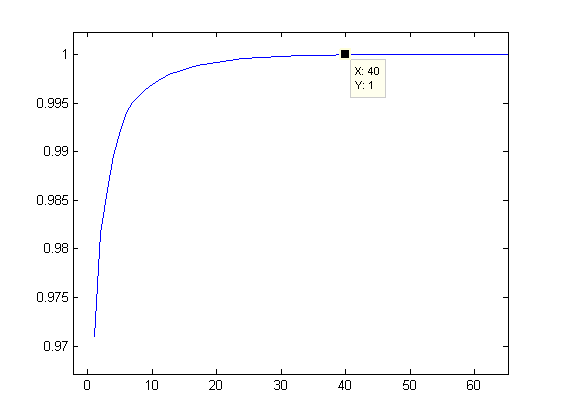
\includegraphics{billeder/pca-on-our-data}
\caption{3D to 2D pca illustration}
\label{fig:pca-on-our-data}
\end{figure}

\subsection{Fisher}

Introtext\\

Math\\

How we use it or why we don't use it\\

Intermediate result\\

%------------------------------------------------



%------------------------------------------------
\section{Discussion}
When looking at the results from table \ref{tab:restest}, it is easy to see that the linear methods: Linear classifier and support vector machines, is worse than the probabilistic methods. This is often the case if the classes is not clusterable, which make it hard to draw a good decision bound. The probabilistic methods is quite good in comparison, and the best match is archived by using the artificial neural network method, which only have a 12.41\% error. \\\ \\

Looking at how well the methods was able to classify the training data, as shown in figure \ref{tab:restrain}. It is seen that the support vector machine and the artificial neural network is capable of classifying the data perfectly whit no error. This is often a indication of over fitting, and you must therefore be very cautious whit the results. By making a extensive search in the solution set of these two methods, we found that this was also the best classifier of the test data, which tells us that over fitting was not the case. Instead this is a result of a very small test set, that makes it possible to completely satisfy the training scenario. This makes the classifiers very specialized. \\\ \\


When looking how the different classifiers perform on the different classes, it is shown that Rune is the one that is generally hardest to recognize. Only in the supervised Gaussian mixture model is this different where Rasmus is the hardest.  It is also seen that for the linear and Discriminative classifier, Rasmus is the easiest to find, but for the other models it is Nicolai. \\\ \\

All the presented methods in table \ref{tab:restest} is able to do classification of a speaker, since there are way more correct guesses than wrong. This can also be seen in figure \ref{fig:talktest}. It is also easy to see from this figure that support vector machines only struggle to classify Rune, but have no problem whit Nicolai and Rasmus. Figure \ref{tab:restest} also shows that the errors for the neural network is not happening in bursts, and is therefore filtered out \\\ \\

Looking at the PCA reduction in figure \ref{fig:DimError} it is seen how the error rate seems to stabilize at 30 features, regardless of algorithm used.


\section{Conclusion}
Using the a MFCC transformation of the audio data, we ware able to get some representative features fore who is speaking. The classification was also tried on features only extracted from the frequency using a FFT. But the MFCC features was way superior to these, so in order to get the simplest model, the FFT features was removed. \\\ \\

In order to further simplify the model, was dimensionality reduction used. Two method of dimensionality reduction was tried PCA and the Fisher method. Even though Fisher theoretically gives the best separation between the classes, does it have the limitation of only reducing to k-1 features. Since we in this project only have three classes, this means we max can get two features. This turns out to be too few classes to do a good classification. Using the PCA reduction to is found that more than 30 PCA reduced features gives the best classification.  \\\ \\ 

In the project have a range of linear, probabilistic and sequential models been used to create a speaker recognition system. It is found that due to the lag of sequential dependency in the features, is the sequential model not suitable for this kind of application. Where the linear and probabilistic models all yields good results. The worst classifier found is the linear classifier that 22.22\% error. Event though this is the one that preforms the worst, it is also the most simple to train and use. The best classifier found was the artificial neural network which only have an error rate on 12.41\%. Compared to the linear classifier is this a very hard to train, but is relative easy to use, when trained. \\\ \\  

When looking at the test result it is clear that the fairly small dataset have had a impact on the performance, and for training a similar application for commercial use way more data is needed. 


%----------------------------------------------------------------------------------------
%	REFERENCE LIST
%----------------------------------------------------------------------------------------

\begin{thebibliography}{99} % Bibliography - this is intentionally simple in this template

\bibitem[Figueredo and Wolf, 2009]{Figueredo:2009dg}
Figueredo, A.~J. and Wolf, P. S.~A. (2009).
\newblock Assortative pairing and life history strategy - a cross-cultural
  study.
\newblock {\em Human Nature}, 20:317--330.
 
\end{thebibliography}

%----------------------------------------------------------------------------------------

\end{multicols}

\end{document}